\documentclass{article}
\usepackage{gvv-book}
\usepackage{gvv}
\usepackage{amsmath}
\usepackage{amsfonts}
\usepackage{tikz}
\usepackage{setspace}
\usepackage{gensymb}
\usepackage[cmex10]{amsmath}
\usepackage{amsthm}
\usepackage{mathrsfs}
\usepackage{txfonts}
\usepackage{stfloats}
\usepackage{bm}
\usepackage{cite}
\usepackage{cases}
\usepackage{subfig}
\usepackage{longtable}
\usepackage{multirow}
\usepackage{enumitem}
\usepackage{mathtools}
\usepackage{tikz}
\usepackage{circuitikz}
\usepackage{verbatim}
\usepackage[breaklinks=true]{hyperref}
\usepackage{tkz-euclide}
\usepackage{listings}
\usepackage{color}    
\usepackage{array}    
\usepackage{longtable}
\usepackage{calc}     
\usepackage{multirow} 
\usepackage{hhline}   
\usepackage{ifthen}   
\usepackage{lscape}     
\usepackage{chngcntr}
\usepackage{graphicx}
\usepackage{float}
\usepackage{multicol}
\usepackage[a4paper, left = 1.5cm, right = 1.5cm]{geometry}

\begin{document}

\begin{center}
\large
    \textbf{ASSIGNMENT 3: GATE 2015 \\ AE : AEROSPACE ENGINEERING}\\
    AI25BTECH11029 - Samyak Gondane
\end{center}



\begin{enumerate}

\item Choose the appropriate word/phrase, out of the four options given below, to complete the following sentence:\\
Apparent lifelessness \underline{\hspace{2cm}} dormant life.
\begin{multicols}{4}
\begin{enumerate}
\item harbours   
\item leads to   
\item supports   
\item affects
\end{enumerate}
\end{multicols}

\item Fill in the blank with the correct idiom/phrase.\\
That boy from the town was a \underline{\hspace{2cm}} in the sleepy village.
\begin{multicols}{4}
\begin{enumerate}
\item dog out of herd
\item sheep from the heap
\item fish out of water
\item bird from the flock
\end{enumerate}
\end{multicols}

\item Choose the statement where underlined word is used correctly.
\begin{enumerate}
\item When the teacher eludes to different authors, he is being elusive.
\item When the thief keeps eluding the police, he is being elusive.

\item Matters that are difficult to understand, identify or remember are allusive.
\item Mirages can be allusive, but a better way to express them is illusory.
\end{enumerate}

\item Tanya is older than Eric.\\
Cliff is older than Tanya.\\
Eric is older than Cliff.\\
If the first two statements are true, then the third statement is:

\begin{multicols}{4}
\begin{enumerate}
\item True
\item False
\item Uncertain
\item Data insufficient
\end{enumerate}
\end{multicols}

\item Five teams have to compete in a league, with every team playing every other team exactly once, before going to the next round. How many matches will have to be held to complete the league round of matches?
\begin{multicols}{4}
\begin{enumerate}
\item 20
\item 10
\item 8
\item 5
\end{enumerate}
\end{multicols}

\item Select the appropriate option in place of underlined part of the sentence.
Increased productivity necessary reflects greater efforts made by the employees.
\begin{enumerate}
\item Increase in productivity necessary
\item Increase productivity is necessary
\item Increase in productivity necessarily
\item No improvement required
\end{enumerate}

\item Given below are two statements followed by two conclusions. Assuming these statements to be true, decide which one logically follows.\\
Statements:\\
\begin{enumerate}
    \item No manager is a leader.
    \item All leaders are executives.
\end{enumerate}
Conclusions:
\begin{enumerate}
    \item No manager is an executive.
    \item No executive is a manager.
\end{enumerate}
\begin{enumerate}
\item Only conclusion I follows.
\item Only conclusion II follows.
\item Neither conclusion I nor II follows.
\item Both conclusions I and II follow.
\end{enumerate}

\item In the given figure angle Q is a right angle, PS:QS = 3:1, RT:QT = 5:2 and PU:UR = 1:1. If area of triangle QTS is 20 $cm^2$, then the area of triangle PQR in $cm^2$ is \underline{\hspace{2cm}}.
\begin{figure}[H]
    \centering
    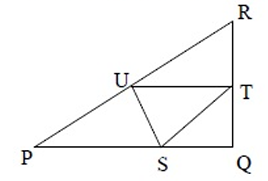
\includegraphics[width=0.3\linewidth]{figs/q8.png}
    \caption{}
    \label{fig:q8}
\end{figure}

\item Right triangle PQR is to be constructed in the xy-plane so that the right angle is at P and line PR is parallel to the x-axis. The x and y coordinates of P, Q, and R are to be integers that satisfy the inequalities: $$-4 ≤ x ≤ 5$ and $6 ≤ y ≤ 16$. How many different triangles could be constructed with these properties?
\begin{multicols}{4}
\begin{enumerate}
\item 110
\item 1100
\item 9900
\item 10000
\end{enumerate}
\end{multicols}

\item A coin is tossed thrice. Let X be the event that head occurs in each of the first two tosses. Let Y be the event that a tail occurs on the third toss. Let Z be the event that two tails occur in three tosses. Based on the above information, which one of the following statements is TRUE?
\begin{enumerate}
\item X and Y are not independent
\item Y and Z are dependent
\item Y and Z are independent
\item X and Z are independent
\end{enumerate}

\item The partial differential equation $\delta u/ \delta t + (u^2/2) = 0$ is
\begin{enumerate}
\item linear and first order
\item linear and second order
\item non-linear and first order
\item non-linear and second order
\end{enumerate}

\item The system of equations for the variables $x$ and $y$
\begin{align}
    a x + b y = e\\
    c x + d y = f
\end{align}
has a unique solution only if
\begin{multicols}{4}
\begin{enumerate}
\item a d - b c ≠ 0
\item a c - b d ≠ 0
\item a + c ≠ b + d
\item a - c ≠ b - d 
\end{enumerate}
\end{multicols}

\item A linear mass-spring-dashpot system is over-damped. In free vibration, this system undergoes
\begin{enumerate}
\item non-oscillatory motion
\item random motion
\item oscillatory and periodic motion
\item oscillatory and non-periodic motion
\end{enumerate}

\item A cantilever with thin-walled channel cross section is subjected to a lateral force at its shear center. The cantilever undergoes
\begin{enumerate}
\item bending without twisting
\item bending and twisting
\item neither bending nor twisting
\item twisting without bending
\end{enumerate}

\item The two non-zero principal stresses at a point in a thin plate are σ₁ = 25 MPa and σ₂ = -25 MPa. The maximum shear stress (in MPa) at this point is \underline{\hspace{2cm}}.

\item Consider the density and altitude at the base of an isothermal layer in the standard atmosphere to be ρ₁ and h₁, respectively. The density variation with altitude (ρ versus h) in that layer is governed by (R: specific gas constant, T: temperature, g₀: acceleration due to gravity at sea level)
\begin{multicols}{4}
\begin{enumerate}
\item $\rho/\rho_1$ = $e^{[-(g₀/RT)(h-h₁)]}$
\item $\rho/\rho_1$ = $e^{[-(g₀/RT)(h₁-h)]}$
\item $\rho/\rho_1$ = $e^{[-(RT/g₀)(h-h₁)]}$
\item $\rho/\rho_1$ = $e^{[-(RT/g₀)(h₁-h)]}$
\end{enumerate}
\end{multicols}

\item For constant free stream velocity and density, a change in lift for a large aspect ratio straight wing, with thin cambered airfoil section at small angles of attack, leads to
\begin{enumerate}
\item a shift of the aerodynamic center and no shift of the center of pressure
\item a shift of the center of pressure and no shift of the aerodynamic center
\item shift of both the aerodynamic center and the center of pressure
\item no shift either of the aerodynamic center or of the center of pressure
\end{enumerate}

\item Which one of the following modes of a stable aircraft has non-oscillatory response characteristics?
\begin{multicols}{4}
\begin{enumerate}
\item Short period
\item Phugoid
\item Dutch roll
\item Spiral
\end{enumerate}
\end{multicols}

\item As a candidate for a vertical tail, which one of the following airfoil sections is appropriate?

\begin{multicols}{4}
\begin{enumerate}
\item NACA 0012
\item NACA 2312
\item NACA 23012
\item Clarke Y profile 
\end{enumerate}
\end{multicols}

\item The primary purpose of a trailing edge flap is to

\begin{multicols}{4}
\begin{enumerate}
\item avoid flow separation
\item increase Cₗ,max
\item reduce wave drag
\item reduce induced drag
\end{enumerate}
\end{multicols}

\item Which one of the following aero engines has the highest propulsive efficiency?
\begin{enumerate}
\item Turbojet engine without afterburner
\item Turbojet engine with afterburner
\item Turbofan engine
\item Ramjet engine 
\end{enumerate}

\item The stoichiometric fuel-to-air ratio in an aircraft engine combustor varies with the compressor pressure ratio as follows:
\begin{multicols}{4}
\begin{enumerate}
\item increases linearly
\item decreases linearly
\item is independent
\item increases nonlinearly
\end{enumerate}
\end{multicols}

\item A rocket engine produces a total impulse of 112 kN·s in a burn time period of 3.5 minutes with a propellant mass flow rate of 0.25 kg/s. The effective exhaust velocity (in m/s) of gas ejecting from the engine is \underline{\hspace{2cm}}.


\item The function $y = x^3 - x$ has

\begin{multicols}{4}
\begin{enumerate}
\item no inflection point
\item one inflection point
\item two inflection points
\item three inflection points
\end{enumerate}
\end{multicols}

\item A $0.5 kg$ mass is suspended vertically from a point fixed on the Earth by a spring having a stiffness of $5 N/mm$. The static displacement (in mm) of the mass is \underline{\hspace{2cm}}.


\item A slender structure is subjected to four different loading cases (I, II, III and IV) as shown below (Figures not to scale). Which pair of cases results in identical stress distribution at section S - S located far away from both ends?

\begin{multicols}{4}
\begin{enumerate}
\item I and II
\item II and III
\item III and IV
\item IV and I
\end{enumerate}
\end{multicols}

\item An aircraft in level and unaccelerated flight with a velocity of $V_\infty = 300 m/s$ requires a power of $9 × 10⁶ W$. If the aircraft weighs $1.5 × 10⁵ N$, the lift-to-drag ratio $L/D$ is \underline{\hspace{2cm}}.


\item The percentage change in the lift-off distance for a 20 percent increase in aircraft weight is \underline{\hspace{2cm}}.


\item Consider a monoplane wing and a biplane wing with identical airfoil sections, wingspans and incidence angles in identical conditions in a wind tunnel. As compared to the monoplane, the biplane experiences
\begin{enumerate}
\item a higher lift and a higher drag
\item a higher lift and a lower drag
\item a lower lift and a lower drag
\item a lower lift and a higher drag
\end{enumerate}

\item A statically stable trimmed aircraft experiences a gust and the angle of attack reduces momentarily. As a result, the center of pressure of the aircraft

\begin{multicols}{4}
\begin{enumerate}
\item shifts forward
\item shifts rearward
\item does not shift
\item coincides with the neutral point
\end{enumerate}
\end{multicols}

\item Consider a wing of elliptic planform, with its aspect ratio AR \longrightarrow \infty. Its lift-curve slope, $dC_1/dx$ = \underline{\hspace{2cm}}.


\item An ideal gas in a reservoir has a specific stagnation enthalpy of h₀. The gas is isentropically expanded to a new specific stagnation enthalpy of $h_\circ/2$ and velocity u. The flow is one-dimensional and steady. Then $u^2/h_\circ$ = \underline{\hspace{2cm}}.


\item The Reynolds number, Re is defined as U∞L/ν where L is the length scale for a flow, U∞ is its reference velocity and ν is the coefficient of kinematic viscosity. In the laminar boundary layer approximation, comparison of the dimensions of the convection term u∂u/∂x and the viscous term $ν\delta^2u/\delta x^2$ leads to the following relation between the boundary layer thickness $\delta$ and Re:

\begin{multicols}{4}
\begin{enumerate}
\item $\delta \propto \sqrt{Re}$
\item $\delta \propto 1/\sqrt{Re}$
\item $\delta \propto Re$
\item $\delta \propto 1/Re$
\end{enumerate}
\end{multicols}

\item Isentropic efficiencies of an aircraft engine operating at typical subsonic cruise conditions with the following components - intake, compressor, turbine and nozzle - are denoted by $\eta_i$, $\eta_c$, $\eta_t$ and $\eta_n$, respectively. Which one of the following is correct?

\begin{multicols}{4}
\begin{enumerate}
\item $\eta_i$ < $\eta_c$ < $\eta_t$ < $\eta_n$
\item $\eta_t$ < $\eta_i$ < $\eta_c$ < $\eta_n$
\item $\eta_c$ < $\eta_t$ < $\eta_i$ < $\eta_n$
\item $\eta_c$ < $\eta_t$ < $\eta_n$ < $\eta_i$
\end{enumerate}
\end{multicols}

\item A rocket nozzle is designed to produce maximum thrust at an altitude, $H = 8 km$ from the sea level. The nozzle operates in

\begin{enumerate}
\item under-expanded condition for $H > 8 km$
\item under-expanded condition for $H < 8 km$
\item sonic exit condition for $H > 8 km$
\item unchoked condition for $H < 8 km$
\end{enumerate}

\item In the solution of $d^2y/dx^2 - 2dy/dx + y = 0$, if the values of the integration constants are identical and one of the initial conditions is specified as $y(0) = 1$, the other initial condition $y'(0)$ = \underline{\hspace{2cm}}.


\item For $x > 0$, the general solution of the differential equation $dy/dx = 1 - 2y$ asymptotically approaches \underline{\hspace{2cm}}.


\item For a parabola defined by $y = ax^2 + bx + c, a \neq 0$, the coordinates $$(x, y)$ of the extremum are

\begin{multicols}{4}
\begin{enumerate}
\item (-b/2a + √(b²-4ac)/2a, 0)
\item (-b/2a, (-b²+4ac)/2a)
\item (-b/2a, (-b²+4ac)/4a)
\item (0, c)
\end{enumerate}
\end{multicols}

\item The 2-D stress state at a point P in the x-y coordinate system is $$[60 50; 50 -40] MPa$. The magnitude of the tangential stress $$(in MPa)$ on a surface normal to the x-axis at P is \underline{\hspace{2cm}}.


\item A cube made of a linear elastic isotropic material is subjected to a uniform hydrostatic pressure of $100 N/mm^2$. Under this load, the volume of the cube shrinks by $0.05$ percent. The Young's modulus of the material, $E = 300 GPa$. The Poisson's ratio of the material is \underline{\hspace{2cm}}.


\item A massless cantilever beam PQ has a solid square cross section $(10 mm × 10 mm)$. This beam is subjected to a load W through a rigid massless link at the point Q, as shown below (figure not to scale). If the Young's modulus of the material $E = 200 GPa$, the deflection $(in mm)$ at point Q is \underline{\hspace{2cm}}.



\item An aircraft, with a wing loading $W/S = 500 N/m^2$, is gliding at $(L/D)max = 10$ and $C_1 = 0.69$. Considering the free stream density $\rho_\infty = 0.9 kg/m^3$, the equilibrium glide speed (in m/s) is \underline{\hspace{2cm}}.


\item For a thin flat plate at $2$ degrees angle of attack, the pitching moment coefficient about the trailing edge is \underline{\hspace{2cm}}.


\item A satellite is to be transferred from its geostationary orbit to a circular polar orbit of the same radius through a single impulse out-of-plane maneuver. The magnitude of the change in velocity required is \underline{\hspace{2cm}} times the magnitude of the escape velocity.


\item A planetary probe is launched at a speed of $200 km/s$ and at a distance of $71,400 km$ from the mass center of its nearest planet of mass $1.9 × 10^{28} kg$. The universal gravitational constant, $G = 6.67 × 10^{-11} m^3/kg·s^2$. The ensuing path of the probe would be

\begin{multicols}{4}
\begin{enumerate}
\item elliptic
\item hyperbolic
\item parabolic
\item circular
\end{enumerate}
\end{multicols}

\item The velocity profile of an incompressible laminar boundary layer over a flat plate developing under constant pressure is given by $u(y)/U_\infty = (3y/2\delta) - (1/2)(y/\delta)^3$. The freestream velocity $U_\infty = 10 m/s$ and the dynamic viscosity of the fluid $\mu = 1.8 \times 10^{-5} kg/ms$. At a streamwise station where the boundary layer thickness $\delta = 5 mm$, the wall shear stress is \underline{\hspace{2cm}} $\times 10^{-3} Pa$.


\item The Pitot tube of an aircraft registers a pressure $\rho_\circ = 54051 N/m^2$. The static pressure, density and the ratio of specific heats of the freestream are $\rho_\infty = 45565 N/m^2$, $\rho_\infty = 0.6417 kg/m^3$ and $\gamma = 1.4$, respectively. The indicated airspeed $(in m/s)$ is

\begin{multicols}{4}
\begin{enumerate}
\item 157.6
\item 162.6
\item 172.0
\item 182.3
\end{enumerate}
\end{multicols}

\item Consider a $NACA 0012$ aerofoil of chord c in a freestream with velocity $V_\infty$ at a non-zero positive angle of attack $\alpha$. The average time-of-flight for a particle to move from the leading edge to the trailing edge on the suction and pressure sides are $t_1$ and $t_2$, respectively. Thin aerofoil theory yields the velocity perturbation to the freestream as $V_\infty(1+\cos\theta)\alpha/\sin\theta$ on the suction side and as $-V_\infty(1+\cos\theta)\alpha/\sin\theta$ on the pressure side, where $\theta$ corresponds to the chordwise position, $x = c/2(1-\cos\theta)$. Then $t_2 - t_1$ is

\begin{multicols}{4}
\begin{enumerate}
\item $-8\pi\alpha c/V_\infty(4-\pi^2\alpha^2)$
\item 0
\item $4\pi\alpha c/V_\infty(4-\pi^2\alpha^2)$
\item $8\pi\alpha c/V_\infty(4-\pi^2\alpha^2))$ 
\end{enumerate}
\end{multicols}

\item Air enters an aircraft engine at a velocity of $180 m/s$ with a flow rate of $94 kg/s$. The engine combustor requires $9.2 kg/s$ of air to burn $1 kg/s$ of fuel. The velocity of gas exiting from the engine is $640 m/s$. The momentum thrust $(in N)$ developed by the engine is

\begin{multicols}{4}
\begin{enumerate}
\item 43241
\item 45594
\item 47940
\item 49779
\end{enumerate}
\end{multicols}

\item A solid rocket motor is designed with a cylindrical end-burning propellant grain of length $1 m$ and diameter $32 cm$. The density of the propellant grain is $1750 kg/m^3$. The specific impulse of the motor is $190 s$ and the acceleration due to gravity is $9.8 m/s^2$. If the propellant burns for a period of $150 s$, then the thrust $(in N)$ produced by the rocket motor is \underline{\hspace{2cm}}.


\item A liquid propellant rocket has the following component masses:
Mass of payload = $180 kg$
Mass of fuel = $470 kg$
Mass of oxidizer = $1170 kg$
Mass of structures = $150 kg$
Mass of guidance systems = $20 kg$
The effective exhaust velocity is $3136 m/s$. The velocity increment $(in km/s)$ of the rocket at burnout, while operating in outer space, is \underline{\hspace{2cm}}.


\item If all the eigenvalues of a matrix are real and equal, then

\begin{enumerate}
\item the matrix is diagonalizable
\item its eigenvectors are not necessarily linearly independent
\item its eigenvectors are linearly independent
\item its determinant is necessarily zero
\end{enumerate}

\item The value of the integral $\int(4x^3 + 3x^2 + 2x + 1) dx$ evaluated numerically using Simpson's rule with one step is

\begin{multicols}{4}
\begin{enumerate}
\item 26.5
\item 26
\item 25.5
\item 25.3
\end{enumerate}
\end{multicols}

\item The following data is for a single degree of freedom system with viscous damping:
mass, m = $10 kg$; spring stiffness, k = $2.25 N/mm$;
damping coefficient, c = $0.0125 N·s/mm$.
The ratio of any two successive amplitudes is \underline{\hspace{2cm}}.


\item Determine the correctness or otherwise of the following assertion [a] and reason [r]:
Assertion [a]: Aircraft directional static stability can be improved by moving the vertical tail rearward.
Reason [r]: Moving the vertical tail rearward increases the moment arm from the tail aerodynamic center to the aircraft center of gravity.
\begin{enumerate}
\item Both [a] and [r] are true and [r] is the correct reason for [a]
\item Both [a] and [r] are true but [r] is not the correct reason for [a]
\item Both [a] and [r] are false
\item [a] is true and [r] is false
\end{enumerate}

\item Consider a 2-D blunt body in an incompressible fluid stream. The flow is irrotational and can be modeled as a linear combination of a uniform flow and a line source (Rankine half body) as shown below. Let s be the distance of the line source from the front stagnation point. Let d be the upstream distance from the stagnation point to the streamwise location (labeled below as P) where the oncoming stream reaches 90 percent of its undisturbed velocity. Then $d/s$ = \underline{\hspace{2cm}}.


\item Following are the operational parameters of an axial compressor stage:
Air mass flow rate = $24 kg/s$
Static temperature of air at the rotor inlet = $278 K$
Velocity of air at the rotor inlet (zero whirl velocity) = $140 m/s$
Work done on the compressor rotor = $734 kJ$
Isentropic efficiency of the compressor stage = $0.86$
Ratio of specific heats = $1.4$
Specific heat at constant pressure = $1.005 kJ/kgK$
The stagnation pressure ratio across the axial compressor stage is \underline{\hspace{2cm}}.

\item The thin rectangular tube shown below is made of a material with shear modulus, $G = 80 GPa$. The shear flow is calculated based on the mid-thickness dimensions. If the free end is allowed to twist no more than $0.0727 rad$, then the maximum torque (in Nm) which the tube can be subjected to at its free end is \underline{\hspace{2cm}}.


\item A $200 mm$ long simply-supported column has a $5 mm \times 10 mm$ rectangular cross section. The Young's modulus of the material, $E = 200 GPa$. Assuming a factor of safety of $2.5$ corresponding to the buckling load, the maximum load (in N) the column can support in compression is \underline{\hspace{2cm}}.


\item For a level flight at cruise altitude, $C_D = 0.018$ with drag coefficient at zero lift, $C_D$,$0 = 0.015$. For a $30\degree$ climb at the same altitude and speed, $C_D = \underline{\hspace{2cm}} \times 10^{-3}$.


\item An aircraft is flying with inertial ground and wind speeds of $v_g^b = (100, 5, 5) m/s$ and $v_w^b = (0, -5, -10) m/s$, respectively, as expressed in the body frame. The corresponding sideslip angle (in degrees) is

\begin{multicols}{4}
\begin{enumerate}
\item 0
\item 5.65
\item 8.49
\item 9.54
\end{enumerate}
\end{multicols}

\item The elliptical area swept by a satellite is $5.6 \times 10^9 km^2$ in one full orbit. Its angular speed is observed to be $0.00125 rad/s$ when it is at a distance of $7,200 km$ from the center of mass of its primary. Its orbital period (in Earth days) is \underline{\hspace{2cm}}.


\item For a normal shock, the relation between the upstream Mach number $(M_1)$ and the downstream Mach number $(M_2)$ is given by $M_2^2 = [(\gamma-1)M_1^2+2]/[2\gamma M_1^2+1-\gamma]$. For an ideal gas with $\gamma = 1.4$, the asymptotic value of the downstream Mach number is \underline{\hspace{2cm}}.


\item  centrifugal air compressor is operating at the following conditions:
Inlet stagnation temperature = $288 K$
Inlet stagnation pressure = $1.15 bar$
Exit stagnation temperature = $454 K$
Exit stagnation pressure = $4.8 bar$
The energy loss due to non-isentropic compression per unit mass of flowing air (ratio of specific heats, $\gamma = 1.4$ and specific heat at constant pressure, $C_p = 1.005 kJ/kgK)$ is \underline{\hspace{2cm}} kJ/kg.

\item Hot gas (ratio of specific heats, $\gamma = 1.33$) at a temperature of $1450 K$ enters into an axial turbine and expands isentropically. Assume that the kinetic energy of the gas across the turbine is negligible. If the ratio of inlet to outlet pressures of the turbine is $9.5$, then the temperature (in K) of gas exiting the turbine is \underline{\hspace{2cm}}.\\
\\
\large
\centering
\textbf{END OF THE QUESTION PAPER}
\end{enumerate}

\end{document}
